\documentclass[doublespacing, 12pt, a4paper]{article}
% Use the option doublespacing or reviewcopy to obtain double line spacing
% \documentclass[doublespacing]{elsart}

% if you use PostScript figures in your article
% use the graphics package for simple commands
%\usepackage{graphics}
% or use the graphicx package for more complicated commands
\usepackage{graphicx,epsfig,tikz}
% or use the epsfig package if you prefer to use the old commands
%\usepackage{epsfig}
% The amssymb package provides various useful mathematical symbols
\usepackage{amssymb,amsmath,mathdots}
\usepackage{setspace}
\usepackage{stmaryrd}
\usepackage{mathtools}
\usepackage[toc,page]{appendix}
\usepackage{hyperref}



% MARGIN SETTINGS
\setlength{\voffset}{-.5in}
\setlength{\textheight}{638pt}
%\setlength{\topmargin}{-0.5in}
\setlength{\textwidth}{6.2in}
\setlength{\oddsidemargin}{-0.in}
\setlength{\evensidemargin}{0in}
\setlength{\footskip}{20pt}


%\usepackage[style=authoryear , backend = biber, maxcitenames=2]{biblatex}

%\addbibresource{GO.bib}

\newcommand{\be}{\begin{equation}}
\newcommand{\en}{\end{equation}}


\def\bga#1\ega{\begin{gather}#1\end{gather}} % suggested in technote.tex
\def\bgas#1\egas{\begin{gather*}#1\end{gather*}}

\def\bal#1\eal{\begin{align}#1\end{align}} % suggested in technote.tex
\def\bals#1\eals{\begin{align*}#1\end{align*}}

\renewcommand{\vec}[1]{\boldsymbol{#1}}

%\newlength{\scalemath}
%\def\scalemath{0.76}

\newcommand*{\Scale}[2][4]{\scalebox{#1}{$#2$}}%
\newcommand{\fhead}{\mathcal C}%
\def \f#1{\fhead \left(#1\right)}%
\def \I#1{\mathcal I \left(#1\right)}%

\newcommand{\p}{\mathcal P}%
\def \bm#1{\mbox{\boldmath{$#1$}}}   % this is used to write boldface Greek
\def \ini#1{\overset{\circ}{ #1}}

\graphicspath{{../images/}}

\doublespacing

\setlength{\topmargin}{0cm} \addtolength{\textheight}{2cm}
\begin{document}
\title{The Freedom to Play GO }
\author{
 Artur L. Gower\\
\small School of Mathematics, University of Manchester, \\
\small Oxford Road, Manchester M13 9PL, UK
}

\date{\today}
\maketitle

\begin{abstract}
Here we use entropy maximisation to calculate the influence of the white stones on the board in the game GO. We are then able to arrive at a simple formula, which leads to efficient algorithms to calculate the total influence of the white stones on the board.
\end{abstract}

\noindent
{\textit{Keywords:} Entropy maximization, Gaming AI, Shortest path}


%%%%%%%%%%%%

\section*{Paths and connectedness}

%%%%%%%%%%%%%
It has been suggested that \href{https://journals.aps.org/prl/abstract/10.1103/PhysRevLett.110.168702}{maximising entropy} is an "intelligent" move in a game. See \href{https://physics.aps.org/articles/v6/46}{Link between Intelligence and Entropy} for a light discussion on the topic.

Here we discuss the influence white has on some empty spot. By that we mean, if white were to place a stone on that empty spot would it be likely to live? To understand this we need ask ourselves how well connected would this white stone be to the other white stones and how close is it to the black stones?  We call this potential white stone the \emph{virtual stone}.

We start by considering how well is the virtual stone connected to the other white stones. See Figure~\ref{fig:VirtualWhitePiece} below, where J6 is the virtual piece. How well connected is J6 to K4?
%We call this connectedness the influence that K4 has on $V$.
Perhaps the minimum number of whites stones need to connect J6 to K4 is a good inverse measure of connectedness? So the connection from J6 to K4 would be some function $\f{n}$, where $n$ is the minimum number of stones needed to connect J6 to K4. In Figure~\ref{fig:VirtualWhitePiece} three stones are needed to connect J6 to K4, however this is also the case for Figure~\ref{fig:OneRoute}. Clearly K4 has a greater influence on J6 in Figure~\ref{fig:VirtualWhitePiece} than in Figure~\ref{fig:OneRoute}. The difference is that there are a few ways to connect J6 to K4 in Figure~\ref{fig:VirtualWhitePiece}, where as there is realistically only one available route in Figure~\ref{fig:OneRoute}.
\begin{figure}
\centering
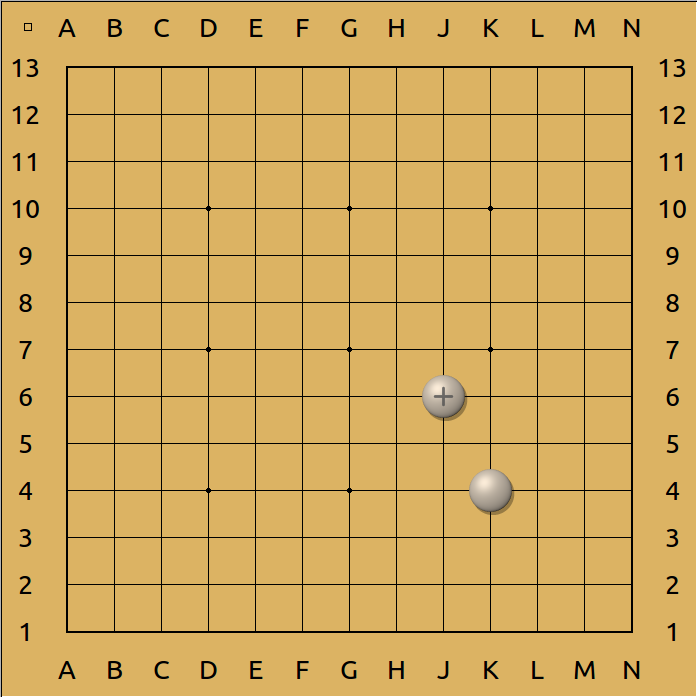
\includegraphics[width=0.4\textwidth]{VirtualWhite}
\caption{How well connected is the virtual stone J6 to K4.}
\label{fig:VirtualWhitePiece}
\end{figure}
\begin{figure}
  \centering
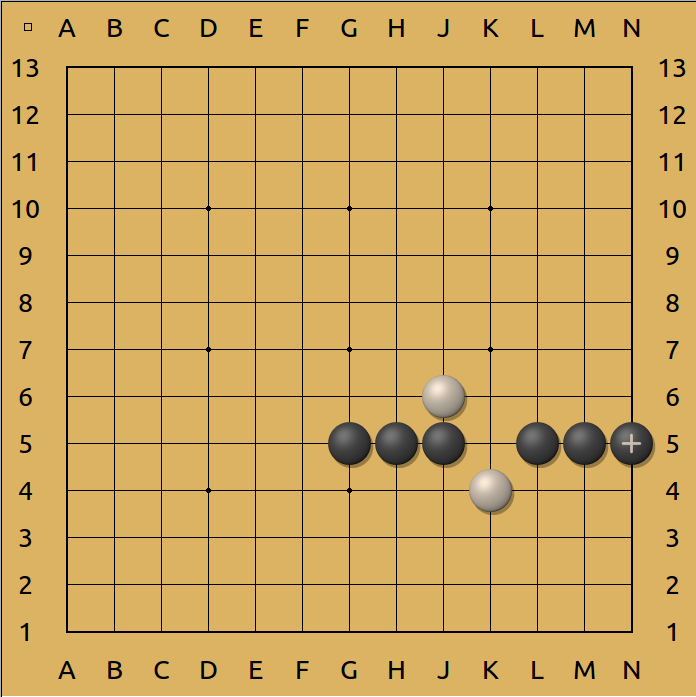
\includegraphics[width=0.4\textwidth]{OneRoute}
\caption{Only one possible route to connect J6 to K4.}
\label{fig:OneRoute}
\end{figure}

The connectedness should consider all the possible routes to connect these two stones, the length of those routes, i.e. the number of stones needed, and how many times these routes cross.

Let each path from J6 to K4 be denoted by $\p = \{s_1, s_2,...\}$, where each $s_j$ is the coordinate of a virtual stone needed to connect J6 to K4. We use $|\p|$ to denote the length of the path.
%a vector $(c_1, c_2, \ldots)$ where the $c_j$'s are the number of stones
How $\fhead$ depends on these paths should be simple, which is vital for both writing a code and being logically consistent. By logical I mean $\fhead$ should be larger
\begin{enumerate}
\item[(i)] the fewer the stones required to connect the virtual stone (i.e. connect J6 to K4).
\item[(ii)] the more paths available to connect the virtual stone.
\item[(iii)] the more potential liberties the virtual stone would have after being connected.
\end{enumerate}
We will use these principals to give a functional form to $\fhead$.

\section*{What are paths?}

How best to define what is a path?
Suppose Figure~\ref{fig:PathThroughWhite} shows the stones in play, in this case we can form a path
$\p = \{J4, H6\}$, see Figure~\ref{fig:PathThroughWhite2}. That is, paths that pass through whites stones already in play do not increase the path length $|\p| =2$. Alternatively, we could form a path $\{K5, K6\}$ which also has length $2$.
\begin{figure}
\centering
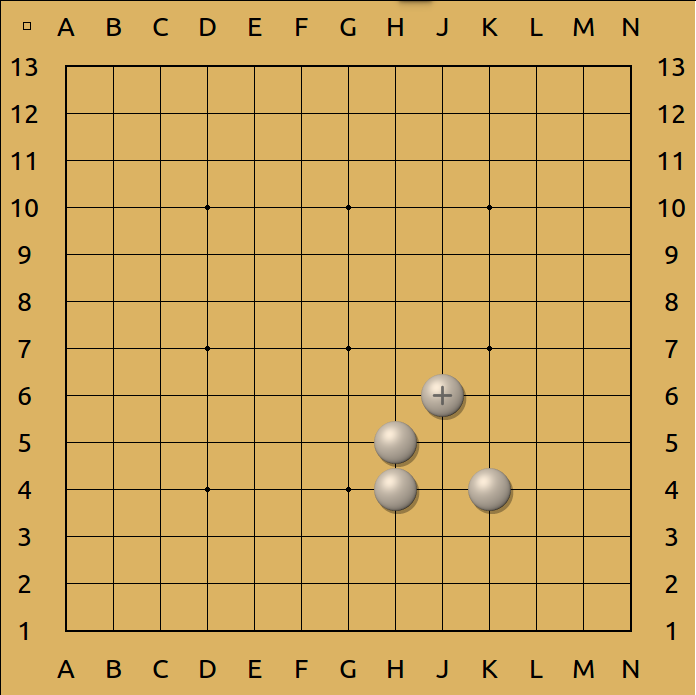
\includegraphics[width=0.4\textwidth]{PathThroughWhite}
\caption{Possible paths to connect J6 and K4?}
\label{fig:PathThroughWhite}
\end{figure}

\begin{figure}
\centering
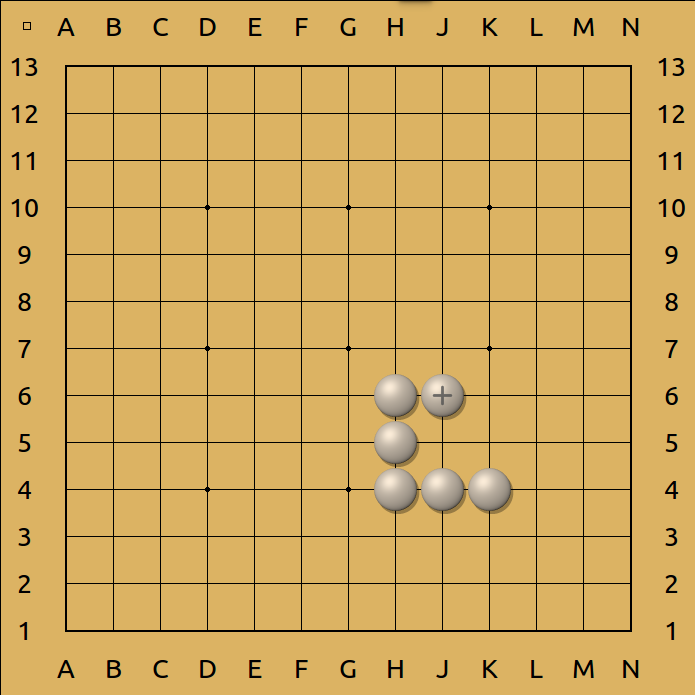
\includegraphics[width=0.4\textwidth]{PathThroughWhite2}
\caption{An example of one path $\p = \{\mathrm{J4},\mathrm{H6}\}$ that connects J6 to K4 in Figure~\ref{fig:PathThroughWhite}}
\label{fig:PathThroughWhite2}
\end{figure}

To eliminate useless paths we define that no path may contain a shorter path. An example of a non-paths is given in Figure~\ref{fig:NonPaths}.  This definition implies that if J6 is already connected to K4 then there are no paths from J6 to K4, except the path with $0$ stones.
\begin{figure}
\centering
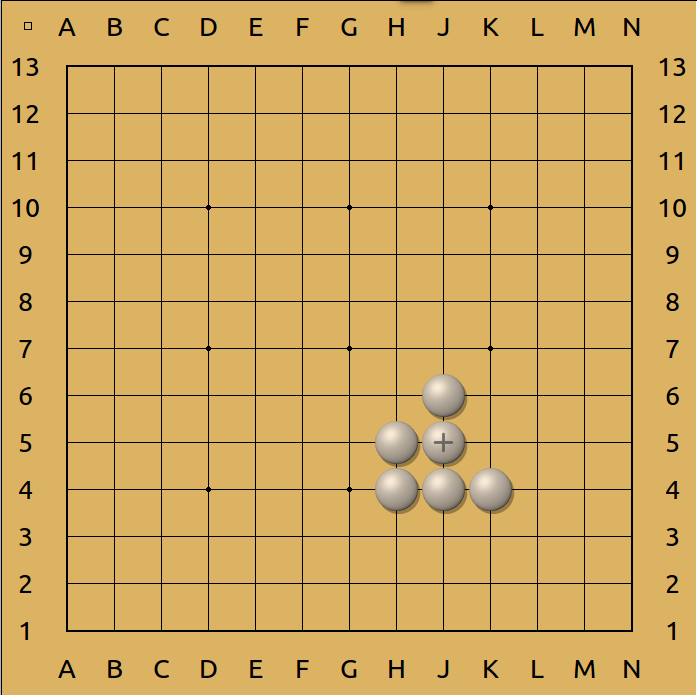
\includegraphics[width=0.4\textwidth]{NonPath1}
\caption{We do not consider that $\{J4,H4,H5,J5\}$ is a path that connects K4 and J6, because it contains in it a shorter path $\{J4,J5\}$  }
\label{fig:NonPaths}
\end{figure}
% \begin{figure}
% \centering
% 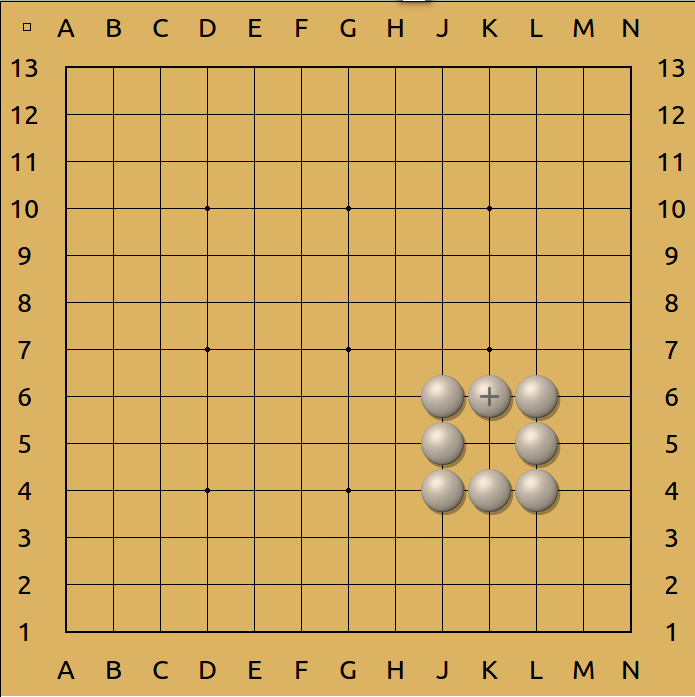
\includegraphics[width=0.4\textwidth]{TwoPaths}
% \caption{Two possible paths}
% \label{fig:TwoPaths}
% \end{figure}

With these definitions of paths, and only considering paths shorter than 5 stones that connect J6 to K4, there are a total of 5 paths in Figure~\ref{fig:VirtualWhitePiece} (note that some of these paths cross), 1 path in Figure~\ref{fig:OneRoute}, and 7 paths in Figure~\ref{fig:PathThroughWhite}.

\section*{Formula for Connectedness $\fhead$}
%Let the paths from the virtual stone to the origin stone be denoted by $\p_j$.
Consider a set of paths $\p_1$, $\p_2$, $\ldots$ that do not cross each other, and all of which connect two stones $O$ (origin stone) and $V$ (virtual stone).
For simplicity, we assume that the total connectedness $\fhead$ of all these (non-intersecting) paths is the sum of the connectedness of each of these paths.
That is we assume linearity
\[
\f{ \cup_j \p_j } = \sum_j \f {\p_j}.
\]
The best way to think about the connectedness is as a probability, from 0 to 1, of how likely two stones are to be connected in the future. The largest value for $\f { \p}$ is when $|\p| = 0$, that is, when two stones are already connected, in which case $\f{ \p} = 1$. The next best possible case is when there are three paths $\p_1$, $\p_2$ and $\p_3$, connecting $V$ to $O$, where each has a length $|\p_j| =1$. In which case we assume $\f{ \p_1 } = \f{ \p_2 } =\f{ \p_3 } = 1/3$, so that
\[
\f{ \p_1 \cup \p_2 \cup \p_3  }= 3 \f{ \p_1 } = 1.
\]
 So we think of $ \f{ \p_1 }$ as being $33\%$ connected. By thinking of connectedness as a probability, we can calculate the connectedness between the two stones in Figure~\ref{fig:2SquareConnected}. For example, we could place stones on both the green squares shown. The probability of this happening is $\f{ \{E4, E5\} } = \f{ \{E4\} } \f{ \{E4\} }  = 1/3^2$.
 \begin{figure}
\centering
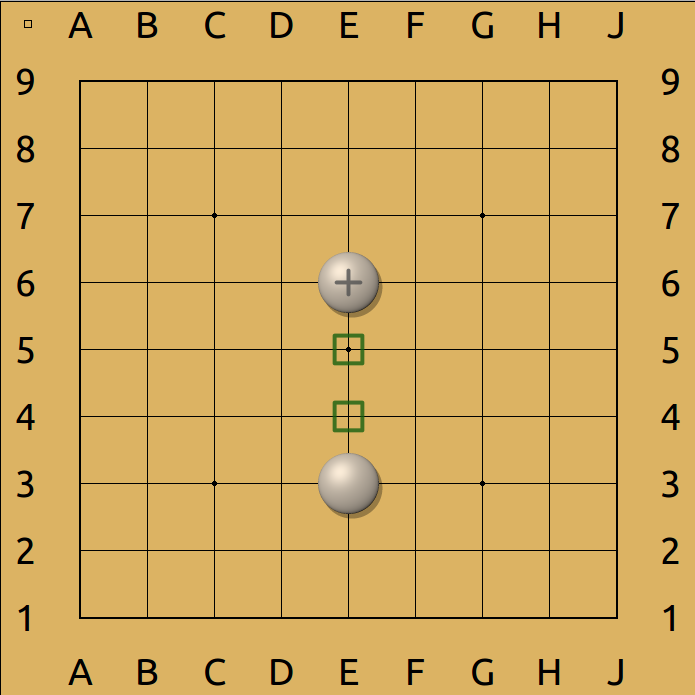
\includegraphics[width=0.4\textwidth]{2SquareConnected}
\caption{What is the probability of these two stones being connected in the future?}
\label{fig:2SquareConnected}
\end{figure}
 This logic can be extended to a path with $n$ stones to conclude that
\be
\f{ \{s_1, s_2, \ldots, s_n\} }  = p^{n},
\label{eqn:Connectiveness}
\en
where $p$ is the probability of connecting one stone, for example $p=1/3$. However, using a value of $p=1/3$ will almost guarantee that the connectedness from one group to some point maybe never be more than $1$, except in exceptional circumstances, such as a group surrounding one point.

%It is possible with this formula to architect examples where the influence of $O$ on $V$ is greater than $1$. When this occurs we cap the influence at $1$.
%Paths that create ladders in favour of white are
%2^{-2}+2^{-1} = 0.75
%2^{-2}+2^{-2} = 0.5
%\[
%\f{ \cup \{2,() \}\cup \{1,() \} } =\f{ \cup \{2,() \}\cup \{3,() \} \cup \{3,() \} }  = 5 M/ 6
%\]
\subsection*{The total influence}

The goal is to estimate the total influence the white stones have on the board. Till now we have talked about connectedness. One path $\p$ contributes to the influence $\I{\p}$ by
\[
\I{\p} = (\text{potential liberties}) \times \f{\p}.
\]
That is, the probability of being connected times the number of total liberties the group would have.
We now redefine a path to be closer to a useful data structure. Let each path be $\p = \{R,n,\vec c\}$, where $n$ is the number of stones, $\vec c$ is called the crossing vector, will be explained later, and
R is the \emph{relative influence}, which we define as
\[
R = (\text{Total liberties of path}) \times \frac{p^n}{n}.
\]
If $\p$ shares no stones with any other path (has no crossing $\vec c = ()$ ), then $\I{\p\{R,n,()\} } = n R$. This formula changes if $\p$ crosses other paths.

Suppose we have two paths that only share one virtual stone with each other. The first path $\p_1 = \{R_1 ,3,\vec c_1\}$ needs 3 stones to be complete and the second path $\p_2 =\{R_2, 2, \vec c_2 \}$ needs two stones. In this case, $\vec c_1 = ([2])$ and $\vec c_2 = ([3])$. The crossing vector $\vec c_1$ has only one element $[2]$ which indicates that only one of its stones is shared with other paths. And because $[2]$ has only one element $2$, means that only one other path crosses through this stone and this path needs in total $2$ stones.
% to connect $V$ to $O$.
An analogous story can be said of $\vec c_2$, that is, it shares only one stone with one other path, and that path needs 3 stones.

Let us look at another example $\p_3 = \{R_3, 4,\vec c_3\}$ with $\vec c_3 =([2,3],[4])$. $\vec c_3$ having two elements $[2,3]$ and $[4]$ means that $\p_3$ has two stones which are shared with other paths. The element $[2,3]$ tells us that $\p_3$ has one stone shared with a path that needs 2 stones and another path that needs 3 stones. The element $[4]$ tells us that $\p_3$ has another stone which is shared only with a path that needs $4$ stones.

Now how do we calculate the influence of $\I{ \p_1 \cup \p_2 \} }$? To make sense, we need
\be
\label{ineq:Crossing}
 \I{ \p_1 } < \I{ \p_2 } < \I{ \p_1 \cup \p_2 } < \I{ \p_1} + \I {\p_2}.
% \I{ \{3,() \} \cup \{2,()\} }.
 %  \f{ \{3,()\} } +\f{ \{2,()\} }
\en
The two inequalities on the left are due to the combined paths $\p_1 \cup \p_2$ being more influential than just one of the paths $\p_1$ or $\p_2$. The last inequality~\eqref{ineq:Crossing}${}_3$ is because these paths share a stone, so they are not as influential as two independent paths (that do not share a stone).
To satisfy all the inequalities~\eqref{ineq:Crossing}, we choose
\be
\I{ \{R_1, 3,([2])\} \cup \{R_2, 2,([3])\} } = \left ( R_1^q + R_2^q \right )^{1/q} + 2 R_1 + R_1,
\en
which satisfies the inequalities for $q>1$ because $0< R_1 < (R_1^q +R_2^q )^{1/q} < R_1 + R_2$. For the influence of $\I{ \{R_1, n_1,([n_2])\} \cup \{R_2, n_2,([n_1])}$ we would replace $ 2 R_1 + R_1$ with $(n_1-1) R_1 + (n_2-1) R_2$.
These formulas were also chosen as they will lead to efficient algorithms. The concept behind this formula is that the path $\p = \{R_1,n,([m])\}$ is not entirely a new path, but can be considered as $n-1$ new stones and one stone which is shared.

Before giving the general formulas, here are some more examples:
\begin{multline*}
  \I{ \{R_1, n_1,([n_2],[n_2])\} \cup \{R_2, n_2,([n_1],[n_1])\} } = 2\left( R_1^q + R_2^q \right)^{1/q}
  \\ + (n_1-2)R_1 + (n_2-2)R_2,
\end{multline*}
\vspace{-2.5cm}

\begin{multline*}
\I{ \{R_1, n_1,([n_3,n_2])\} \cup \{R_2, n_2,([n_1,n_3])\} \cup \{R_3, n_3,([n_1,n_2])\} } = \\
     \left( R_1^q + R_2^q + R_3^q \right)^{1/q}
     + (n_1-1)R_1 + (n_2-1) R_2 + (n_3-1)R_3.
\end{multline*}
Note that all the following limits make sense $R_1 \to \infty$, $R_1 \to 0$, $n_1 \to \infty$, and in particular, when $n_1 =1$, there are no intersection because by definition there is only one path (there can be no paths contained completely inside another path).

To write the general formula it is best to introduce a new notation. We now denote each path by $\p = (R, \vec s)$, where $\vec s$ is the collection of virtual stones (needed to complete the path).
Let $\p_j = (R_j, \vec s^j)$ be all the paths that reach the same arbitrary point.
% The number of elements in $\vec s^q$, denoted by $\|\vec s^q\|$, is the number of stones to complete $\p^q$.
Let $\vec {S} = \cup_j \vec s^j$ be the set of all distinct virtual stones.
For each stone $s \in \vec {S}$, generate a set $\vec R^s$ of the relative influences of all the paths that contain $s$. That is, $R^s_j$ is the relative influence of some path $\p_j$ that needs the virtual stone $s$ to be complete. We can now write the master formula as
\be
\I{ \cup_j \p_j } = \sum_{s \in \vec S} \|\vec R^s\|_q,
\label{eqn:master}
\en
where $||\cdot ||_q$ is the $q$--norm with $q>1$.





\end{document}
\grid
